%=========================================================================
% (c) 2014, 2015 Josef Lusticky

\chapter{Setup}\label{chap:setup}

%=========================================================================
% (c) 2014, 2015 Josef Lusticky

\section{Hardware and networking}\label{sec:setup-hardware}
Figure~\ref{fig:setup-supermicro-board} shows the block diagram of the Supermicro motherboard.
The Intel Xeon E5-2660 v2 processors were plugged into the CPU sockets.
The Mellanox ConnectX-3 EN adpater was plugged into the PCIE 3.0 x8 Upper slot,
which is part of the {\it{WIO}} block.
The PCI-Express links are directly connected to the CPU~1 only.
\begin{figure}
	\centering
	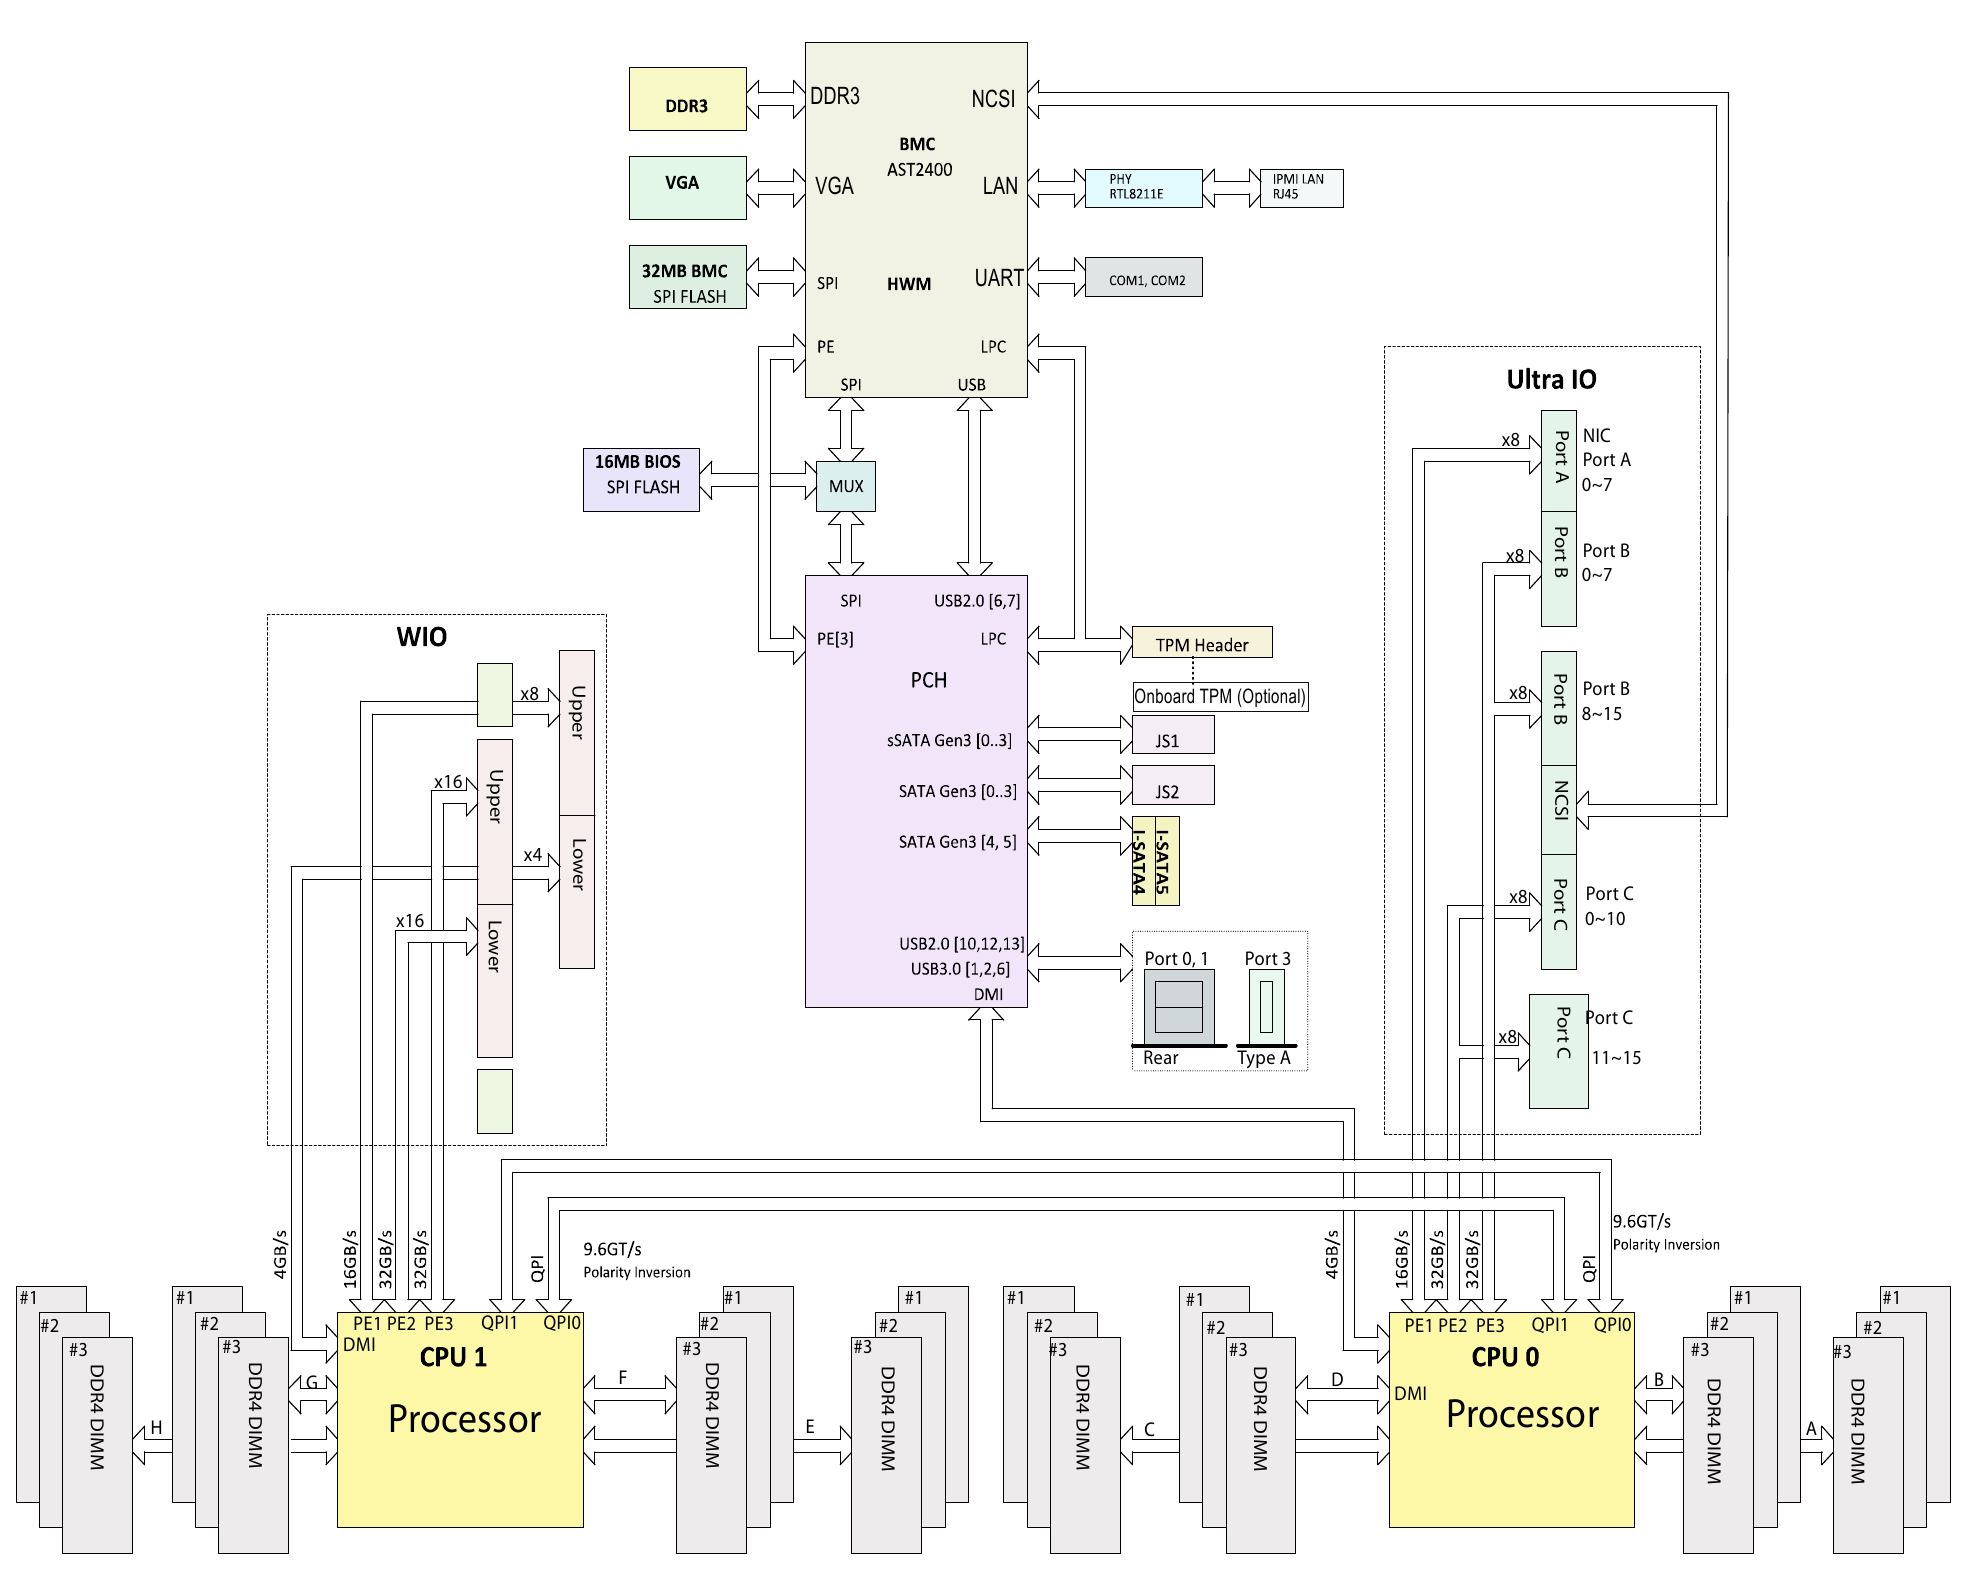
\includegraphics[width=15cm,keepaspectratio]{fig/supermicro-x10drui.png}
	\caption{Supermicro motherboard's block diagram}
	\label{fig:setup-supermicro-board}
\end{figure}

The server was put to the same rack as the Spirent hardware generator.
A pair of 40GBASE-SR4 multimode fiber cables with QSPF connectors
was used to connect Spirent with the Mellanox ConnectX-3 EN adapter.

IPv4 addresses from 192.0.2.0/24 (TEST-NET-1) block were assigned~\cite{rfc5737}.
IPv6 addresses from 2001:db8::/32 range were assigned.
Addresses within these blocks should not appear on the public Internet~\cite{rfc3849}.
Figure~\ref{fig:addressing-scheme} shows the addressing scheme used for the measurements.
\begin{figure}[H]
	\centering
	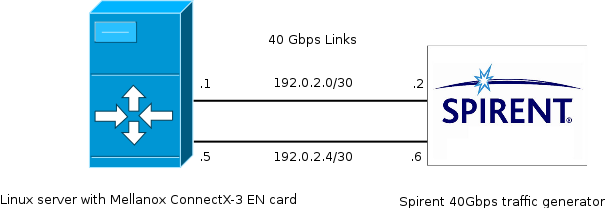
\includegraphics[width=13.5cm,keepaspectratio]{fig/net-setup.png}
	\caption{Addressing scheme}
	\label{fig:addressing-scheme}
\end{figure}



%Enable IPv4 packet forwarding:
%echo 1 > /proc/sys/net/ipv4/ip\_forward


%ip neigh add 1.0.0.2 lladdr f4:52:14:5e:6c:71 dev enp6s0d1
%ip neigh add 2.0.0.2 lladdr f4:52:14:5e:6c:70 dev enp6s0

%ip addr add 1.0.0.1/24 broadcast 1.0.0.255 dev enp6s0d1
%ip addr add 2.0.0.1/24 broadcast 2.0.0.255 dev enp6s0


%Load BGP routes:
%\begin{lstlisting}
%Basic info: size of leaf: 40 bytes, size of tnode: 40 bytes.
%Main:
        %Aver depth:     2.43
        %Max depth:      8
        %Leaves:         503308
        %Prefixes:       538739
        %Internal nodes: 114430
          %1: 58725  2: 26171  3: 14808  4: 7316  5: 4239  6: 2103  7: 1065  8: 2  17: 1
        %Pointers: 995798
%Null ptrs: 378061
%Total size: 61373  kB
%\end{lstlisting}


%=========================================================================
% (c) 2014, 2015 Josef Lusticky

\section{Networking}\label{sec:setup-networking}
Default installation of CentOS with the updates avaliable on 7th January 2015 installed,
including the distribution Linux kernel version 3.10.0-123.13.1.el7.x86\_64.


IPv4 addresses from 192.0.2.0/24 (TEST-NET-1) block were assigned~\cite{rfc5737}.
IPv6 addresses from 2001:db8::/32 range were assigned,
addresses within this block should not appear on the public Internet~\cite{rfc3849}.

Section%~\ref{}
described how the mlx4 drivers set up network interfaces.
In the measurements, IPv4 addresses 1.0.1.1 and 1.0.2.1 with 24-bit subnet mask were assigned to the interfaces.
%These subnets are not part of the BGP routes.
On the Spirent, the corresponding addresses 1.0.1.2 and 1.0.2.2 with 24-bit subnet mask were assigned.
Figure~\ref{fig:measurements-setup} shows the network scheme used for the measurements.
\begin{figure}[H]
	\centering
	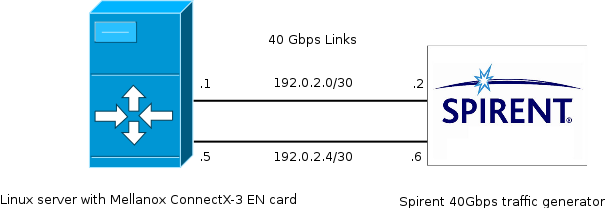
\includegraphics[width=13.5cm,keepaspectratio]{fig/net-setup.png}
	\caption{Measurement setup}
	\label{fig:measurements-setup}
\end{figure}


Enable IPv4 packet forwarding:
echo 1 > /proc/sys/net/ipv4/ip\_forward


ip neigh add 1.0.0.2 lladdr f4:52:14:5e:6c:71 dev enp6s0d1
ip neigh add 2.0.0.2 lladdr f4:52:14:5e:6c:70 dev enp6s0

ip addr add 1.0.0.1/24 broadcast 1.0.0.255 dev enp6s0d1
ip addr add 2.0.0.1/24 broadcast 2.0.0.255 dev enp6s0


Load BGP routes:
\begin{lstlisting}
Basic info: size of leaf: 40 bytes, size of tnode: 40 bytes.
Main:
        Aver depth:     2.43
        Max depth:      8
        Leaves:         503308
        Prefixes:       538739
        Internal nodes: 114430
          1: 58725  2: 26171  3: 14808  4: 7316  5: 4239  6: 2103  7: 1065  8: 2  17: 1
        Pointers: 995798
Null ptrs: 378061
Total size: 61373  kB
\end{lstlisting}


%=========================================================================
% (c) 2014, 2015 Josef Lusticky

\section{Software and firmware}
Base CentOS 7 was installed on the server.
The operating system features Linux kernel based on version 3.10 -
the installed version is 3.10.0-123.20.1.el7.x86\_64.
The operating system was updated with all updates available as of 1st May 2015.
The upstream kernel version 4.0.2 was additionally installed from the ELRepo repository~\cite{elrepo-kernel-ml}.

The Linux kernel detects the Mellanox ConnectX-3 EN card automatically and loads the mlx4\_core and mlx4\_en module.
The mlx4\_core module prints the detected PCI-Express link parameters to the kernel's message buffer.
The buffer can be viewed using the {\it{dmesg}} utility and its partial output is shown bellow:
\begin{lstlisting}[language=TeX]
mlx4_core 0000:06:00.0: PCIe link speed is 8.0GT/s, device supports 8.0GT/s
mlx4_core 0000:06:00.0: PCIe link width is x8, device supports x8
\end{lstlisting}
The mlx4\_core module further registers interrupts and prints the assigned IRQ numbers for each queue
to the kernel's message buffer:
\begin{lstlisting}[language=TeX]
mlx4_core 0000:06:00.0: irq 61 for MSI/MSI-X
mlx4_core 0000:06:00.0: irq 62 for MSI/MSI-X
...
mlx4_core 0000:06:00.0: irq 90 for MSI/MSI-X
\end{lstlisting}

The driver uses either MSI or MSI-X feature of the PCI-Express bus, as described in section~\ref{sec:40gbe-throughput}.
The MSI-X feature is used automatically if the system supports it, otherwise the adapter uses MSI.
The {\it{lspci -vv}} command can be used to check whether MSI-X is used.
Listing~\ref{lst:setup-lspci} shows partial output of lspci for the Mellanox ConnectX-3 EN adapter.
The MSI-X capability is followed by an Enable flag which is followed with either "+" (enabled)
or "-" (disabled).
Listing~\ref{lst:setup-lspci} shows that the system supports MSI-X and the adapter is configured to use it.
\begin{lstlisting}[language=TeX,label={lst:setup-lspci},caption={Partial output of lspci -vv for Mellanox ConnectX-3 EN}]
06:00.0 Ethernet controller: Mellanox Technologies MT27500 Family [ConnectX-3]
		...
		Capabilities: [9c] MSI-X: Enable+ Count=128 Masked-
				...
				LnkCap: Port #8, Speed 8GT/s, Width x8, ASPM L0s, Exit Latency L0s unlimited, L1 unlimited
				...
\end{lstlisting}

Apart from the NIC driver, the Mellanox ConnectX-3 adapter uses its own proprietary firmware.
The firmware was updated to version 2.32.5100, which is the latest version available as of 10th January 2015.
The firmware is not part of the Linux kernel and its update procedure is described in appendix~\ref{app:firmware}.


\section{Software settings}
Change the scaling governor for each CPU present in the system to performance (default is powersave):
\begin{lstlisting}
echo performance | tee /sys/devices/system/cpu/cpu[0-9]*/cpufreq/scaling_governor
\end{lstlisting}
Disable SELinux by editing SELINUX variable in /etc/sysconfig/selinux
(default is enforcing) and reboot the computer to apply:
\begin{lstlisting}
vi /etc/sysconfig/selinux
	SELINUX=disabled
reboot
\end{lstlisting}
%To disable the netfilter completely execute systemctl stop firewalld.
%If disabling the netfilter is not appropriate, flush all chains iptables -F,
%delete all user-defined chains iptables -X (which can be checked again by iptables -L).
Disable netfilter completely:
\begin{lstlisting}[language=TeX]
systemctl stop firewalld
systemctl disable firewalld  # do not execute firewalld on boot
\end{lstlisting}
Enable IPv6 on all interfaces (or at least on the forwarding interfaces):
\begin{lstlisting}
echo 0 > /proc/sys/net/ipv6/conf/all/disable\_ipv6
\end{lstlisting}
Enable IPv4 forwarding:
\begin{lstlisting}
echo 1 > /proc/sys/net/ipv4/ip\_forward
\end{lstlisting}
Enable IPv6 forwarding on all interfaces (or at least on the forwarding interfaces):
\begin{lstlisting}
echo 1 > /proc/sys/net/ipv6/conf/all/forwarding
\end{lstlisting}

IPv4 neighbours:
\begin{lstlisting}
ip neigh add 192.0.2.2 lladdr 00:10:94:00:00:01 dev enp6s0d1
ip neigh add 192.0.2.6 lladdr 00:10:94:00:00:02 dev enp6s0
\end{lstlisting}
IPv6 neighbours:
\begin{lstlisting}
ip -6 neigh add 2001:db8:1::2 lladdr 00:10:94:00:00:03 dev enp6s0d1
ip -6 neigh add 2001:db8:2::6 lladdr 00:10:94:00:00:04 dev enp6s0
\end{lstlisting}

Assign IPv4 addresses:
\begin{lstlisting}
ip addr add 192.0.2.1/30 broadcast 192.0.2.3 dev enp6s0d1
ip addr add 192.0.2.5/30 broadcast 192.0.2.7 dev enp6s0
\end{lstlisting}
Assign IPv6 addresses:
\begin{lstlisting}
ip -6 addr add 2001:db8:1::1/64 dev enp6s0d1
ip -6 addr add 2001:db8:2::5/64 dev enp6s0
\end{lstlisting}

%Additional system settings for a particular measurement are described.
